\chapter{Results}
\label{chap:simulation_results}

In this chapter, we present results for the estimation of actuation configuration for using both simulation data and data from the real system.
Since the parameter space of the motor orientation is not very intuitive, we transform the parameter results (and its variance) to a more intuitive form such that we can compare them.
Concretely speaking, we calculate the estimated motor position in the coordinate frame of the motor at its \textit{true} position.
Since the true position is not known for real system results, we define one estimate as being true (e.g. the mean over all available estimates).
Then we can compare the multiple estimates in this \textit{tangential coordinate frame} $t$.
The error of the actuator arrangement can then be expressed by a distance, which can be approximated by the euclidean norm in the x-y plane of the tangential frame, and an angle, which is the offset between the x axes of the tangential and estimated coordinate frames.
\\
DRAW DISTANCE AND ANGLE INTO IMAGE. INCREASE RESOLUTION. CORRECT COORDINATE LABELS.

\begin{figure}[hbtp]
\centering
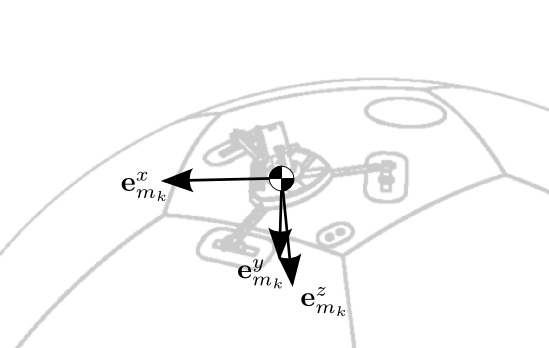
\includegraphics[scale=1]{images/tangential_frame.png}
\caption{The \textit{tangential frame} is the coordinate frame of the motor at its \textit{true} position. If the true position is not known, an estimate is used. In any case, its $\lbrace \mathbf{e}^x_{m_k} , \mathbf{e}^y_{m_k} \rbrace$ plane will be tangential to the spherical hull such that an error of the arrangement can be approximated be the euclidean norm in the .}
\label{fig:tangential_frame}
\end{figure}

BLA BLA BLA
We recorded one large dataset.
Same inputs to simulation.
Split large datasets into multiple datasets ('normal' size) s.t. we have some statistics.

\section{Simulation}
\subsection{Estimation Confidence}
...Show estimate STD
...and explain

... How does STD change when number of inputs changes (you know, this plot...)

\subsection{Convergence Regions}
...That is clear. Add plot and describe

\section{Experiments}
\subsection{Estimation Confidence}
...Copy past from Simulation. Replace STD by RMS. Compare Experiment with Simulation.
...That means do not show a 'you-know-which-plot' again (it will be very similar to the one above)
...But show this angular acceleration plot. Add a error subplot to it.
\subsection{Convergence Regions}
...Same as above
\section{Ground Truth}
...Do not tell toooo much in this section. Nobody likes to read long reports. So just mention 'we did it' and show the results.

...